\documentclass{standalone}
\usepackage{tikz}
\usetikzlibrary{arrows.meta, positioning, shapes, fit}

\begin{document}

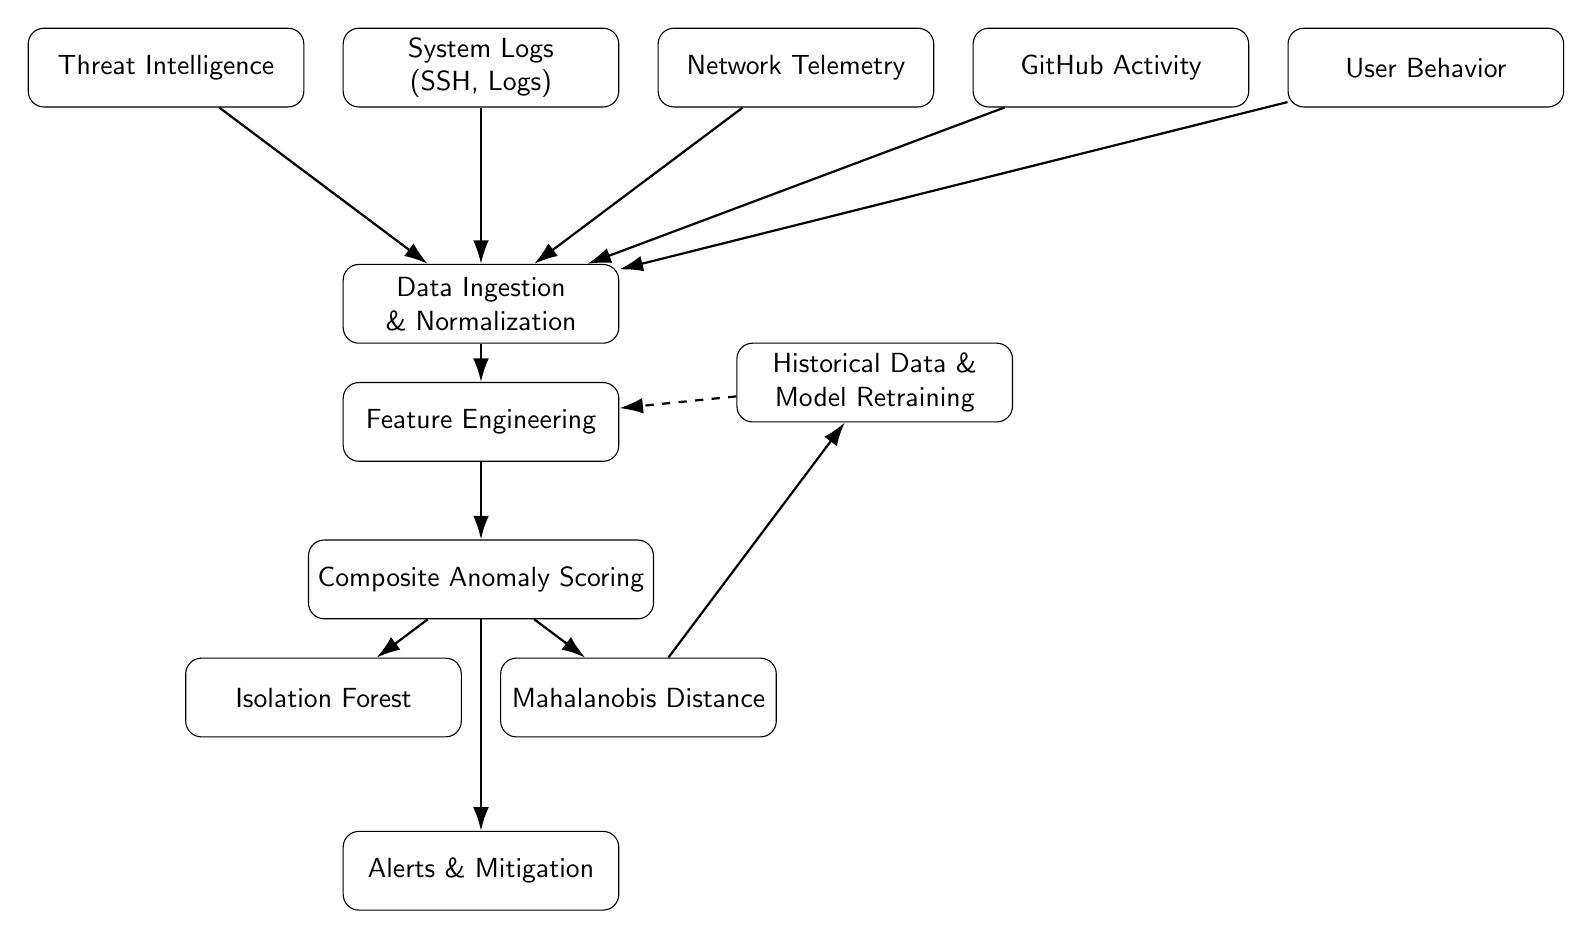
\begin{tikzpicture}[
    font=\sffamily,
    node distance=1.8cm,
    box/.style={
        rectangle, 
        draw=black, 
        fill=white, 
        rounded corners=2mm, 
        align=center, 
        minimum width=3.5cm, 
        minimum height=1cm
    },
    arrow/.style={
        -{Latex[length=3mm,width=2mm]}, 
        thick
    },
    dashedarrow/.style={
        dashed, -{Latex[length=3mm,width=2mm]},
        thick
    }
]

% --- Nodes ---
\node[box] (threatintel) at (1, 10) {Threat Intelligence};
\node[box] (logs) at (5, 10) {System Logs\\(SSH, Logs)};
\node[box] (telemetry) at (9, 10) {Network Telemetry};
\node[box] (github) at (13, 10) {GitHub Activity};
\node[box] (behavior) at (17, 10) {User Behavior};

\node[box] (ingestion) at (5, 7) {Data Ingestion\\ \& Normalization};
\node[box] (feature) at (5, 5.5) {Feature Engineering};
\node[box] (scoring) at (5, 3.5) {Composite Anomaly Scoring};

\node[box] (isolation) at (3, 2) {Isolation Forest};
\node[box] (mahal) at (7, 2) {Mahalanobis Distance};
\node[box] (retrain) at (10, 6) {Historical Data \&\\Model Retraining};
\node[box] (alerts) at (5, -0.2) {Alerts \& Mitigation};

% --- Edges ---
\draw[arrow] (logs) -- (ingestion);
\draw[arrow] (threatintel) -- (ingestion);
\draw[arrow] (telemetry) -- (ingestion);
\draw[arrow] (github) -- (ingestion);
\draw[arrow] (behavior) -- (ingestion);

\draw[arrow] (ingestion) -- (feature);
\draw[arrow] (feature) -- (scoring);
\draw[arrow] (scoring) -- (isolation);
\draw[arrow] (scoring) -- (mahal);
\draw[arrow] (mahal) -- (retrain);
\draw[dashedarrow] (retrain) -- (feature);
\draw[arrow] (scoring) -- (alerts);

\end{tikzpicture}

\end{document}